\section{Deterministic Simulation}
\label{ch:determ_sim}
The traditional way of simulating chemical models is to solve a system of differential equations. The solution obtained is deterministic in the sense that it is, for given parameters, unique and accurately reproducible (up to possible numerical errors). 
\subsection{Reaction Rate Equations}
Let there be a system with species $X_i$, $i=1, \ldots,N$ and reactions $R_j$, $j=1, \ldots,M$. The state of the system $\vec{x}(t)$ at time $t$ is determined by the concentrations\footnote{Unlike in chemical literature where concentration is usually defined as "number of moles/volume", in this thesis a more general concept of concentration scaling is introduced (see chapter \ref{ch:scaling}).} of its species $X_i$. Let $x_i = [X_i]$ denote the concentration of species $X_i$. For the moment, the system is considered to be well-stirred, i.e.\ the system is spatially homogeneous with respect to the concentrations of all species. A spatial effect in inhomogeneous systems, namely diffusion, will be considered in chapter \ref{det_diff}. 

By applying the \textit{Law of mass action}, one can find $N$ differential equations that describe the rate of change of concentration over time for every species $X_i$:
\begin{equation}
\frac{dx_i}{dt} = \sum_{j=1}^M v_{ij}f_j(\vec{x})
\end{equation}
$v_{ij}$ denotes the number of particles of species $X_i$ that are created ($v_{ij} > 0$) or consumed ($v_{ij} < 0$) in reaction $R_j$. $f_j$ is the reaction rate of $R_j$ which in general depends on the current state of the system. 

For simple ("elementary") reactions, the reaction rate is proportional to the product of the concentrations of the reactant species raised to the power of the respective stoichiometric coefficients. Considering for example the reaction $\ce{ 2A -> B}$, one has $\frac{da}{dt} = -2 k a^2$ and $\frac{db}{dt} = k a^2$. 

Applying this formalism to the reactions \eqref{eq:r1} - \eqref{eq:r4} from the Gray-Scott model, the system can be represented by the following differential equations:
\begin{align}
\label{eq:ode1}
\frac{du}{dt} &= - \rho u v^2 + F(1-u) \\
\label{eq:ode2}
\frac{dv}{dt} &= \rho u v^2 - (F + \kappa) v
\end{align}
In order to uniquely determine the solution of the system, the mathematical model is completed by introducing initial conditions:
\begin{equation}
\vec{x}(t = 0) = \vec{x}_0 = \begin{bmatrix}u_0 & v_0\end{bmatrix}^T
%\vec{x}(t = 0) = \vec{x}_0 = \lbrack u_0 \: v_0 \rbrack^T
\end{equation}

\subsection{Steady State Analysis}
Steady state analysis is a practical way to gain an initial insight into how a chemical system may develop in time. In order to better understand the primary example of this thesis, the Gray-Scott model shall now be analyzed with this technique. 

A steady state $\vec{x}_s$ of a system of ordinary differential equations (ODEs) of the form $\frac{d\vec{x}}{dt}=f(\vec{x},t)$ has to satisfy $f(\vec{x}_s,t)=\vec{0} \ \forall t \geq 0$. Considering the equations \eqref{eq:ode1} and \eqref{eq:ode2}, it is obvious that $\vec{x}_{s1} = \begin{bmatrix} 1.0 & 0.0\end{bmatrix}^T$ is a trivial steady state. When all molecules of species V are gone (or there have never been any), the autocatalyzed reaction \eqref{eq:r4} cannot fire any more and the concentration $v$ will remain at zero. The system is therefore reduced to the single ODE $\frac{du}{dt} = F (1-u)$, where the right hand side is 0 iff\footnote{"if and only if"} $u=1$. \\
Throughout the simulations which are carried out in chapter \ref{ch:4}, the parameter values proposed in \cite{rossinelli_accelerated_2008} ($F = 0.04$, $\kappa = 0.06$ and $\rho = 1.0$) will be used. For this setup, another steady state is located at $\vec{x}_{s2} = \begin{bmatrix}0.5 & 0.2\end{bmatrix}^T$. Detailed calculations can be found in the appendix (\ref{ch:app1}). 

To asses the stability of the steady states, the eigenvalues of the Jacobian evaluated at these points in phase space are needed. In the trivial case on obtains $\lambda_{11} = -0.1$ and $\lambda_{12} = -0.04$. Since the real part of both eigenvalues is less than zero (i.e.\ $\Re(\lambda_{1i})<0, i=1,2$), the steady state is stable. The eigenvalues of the non-trivial pole are $\lambda_{21} = 0$ and $\lambda_{22} = 0.02$, in consequence the steady state is unstable. 

Considering initial conditions $\vec{x}_0 = \begin{bmatrix}0.5 & 0.25\end{bmatrix}^T$ and the results of the calculations above one can predict that the system will move towards the steady state $\vec{x}_{s1}$ over time. This behaviour can be observed in figure \ref{fig:gs_time_evolution} after the transient response has gone away. Figure \ref{fig:phasespace} illustrates the corresponding trajectory in phase space. It can be concluded that diffusion is necessary for complex pattern formation in the Gray-Scott model. An advanced analysis of the involved mechanism (i.e.\ Turing bifurcation) can be found in \cite{vastano_turing_1988}. 

\begin{figure}
\centering
%l b r t
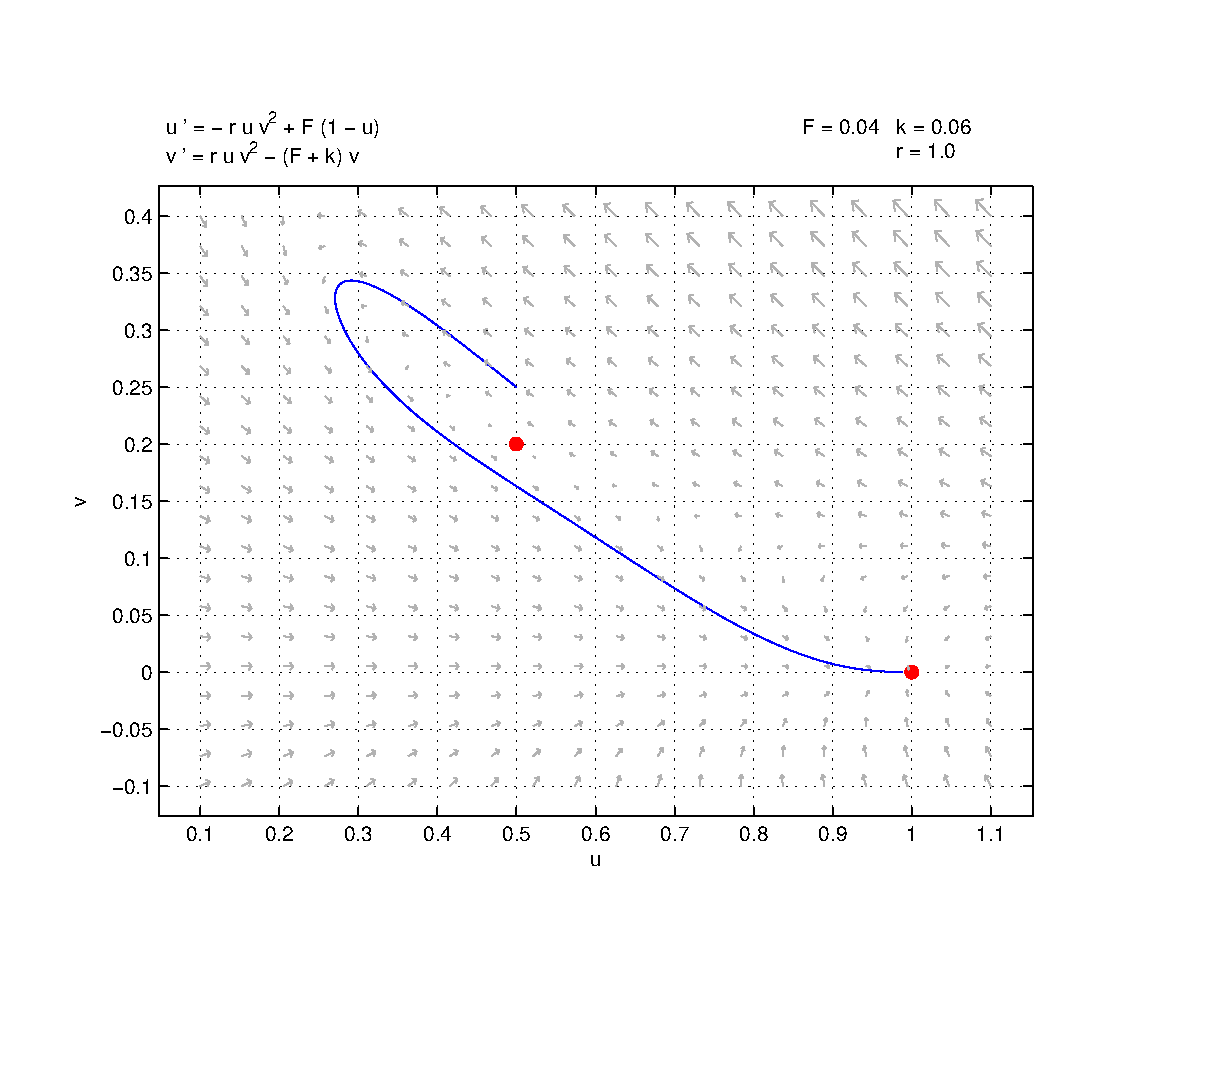
\includegraphics[trim = 5mm 25mm 20mm 5mm, clip, width=3cm,width=\textwidth]{images/phasespace.eps}
\caption{Phase space plot of the Gray-Scott local reaction system. Trajectory starts at $\vec{x}_0$. Red dots mark steady states. }
\label{fig:phasespace}
\end{figure}

%\subsection{Diffusion and Fick's Law}
\subsection{Diffusion and Fick's Law}
\label{det_diff}
The term diffusion describes the phenomenon that matter migrates in the direction of the negative concentration gradient. In consequence, inhomogeneities in the system tend to spread over time and gradients disappear (cite Atkins, pg.\ 770). Diffusion is an integral part of the Gray-Scott model since it is essential for the pattern formation mechanism. In the following, a deterministic description for diffusion (Fick's law) will be derived to incorporate the phenomenon into the reaction rate equations \eqref{eq:ode1} and \eqref{eq:ode2} given above. 

Let there be a cubic tube filled with a solution of some species A. The tube stretches along the $x$-Axis. The extent in the two other directions is negligibly small and so are possible concentration inhomogeneities in this plane. On the left end, the concentration $a = [A]$ is high, on the right end it is low. Figure \eqref{fig:fickslaw} illustrates the setup. Considering a slab of length $l$ ranging from $x_s$ to $x_s + l$ perpendicular to the $x$-Axis, the change of concentration inside the slab in some infinitesimal time interval is equal to the influx through the cross-sectional area $A$ at $x = x_s$ minus the flux out of the slab at $x = x_s + l$:
\begin{align}
\label{eq:diff_flux}
\frac{\partial a}{\partial t} = \frac{J(x_s) A dt}{A l dt} - \frac{J(x_s + l) A dt}{A l dt} = \frac{J - J'}{l}
\end{align}
The flux $J(x)$ at position $x$ is proportional to the negative concentration gradient $\frac{\partial a}{\partial x}$ at $x$. Using this relation gives 
\begin{align}
\begin{split}
J - J' &= -D \frac{\partial a}{\partial x} + D \frac{\partial a'}{\partial x} \\
&= -D \frac{\partial a}{\partial x} + D \frac{\partial}{\partial x} \left\{ a + \frac{\partial a}{\partial x} l \right\} 
= D l \frac{\partial^2 a}{\partial x^2}
\end{split}
\end{align}
with positive diffusion constant $D$. 

\begin{figure}
\centering
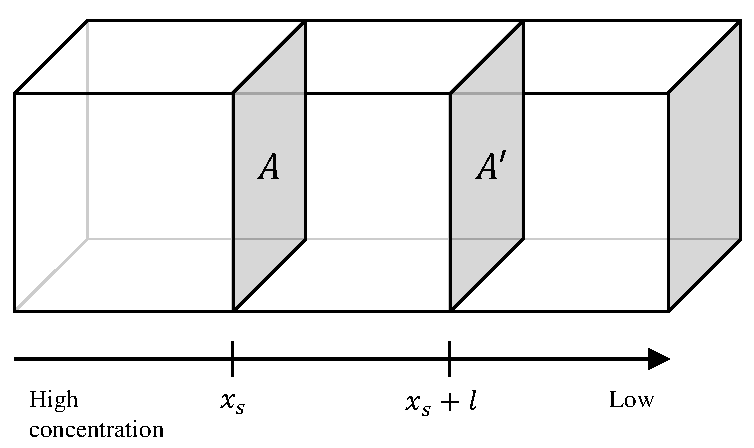
\includegraphics[width=\textwidth]{images/fickslaw.pdf}
\caption{Illustration of the setup used to derive Fick's law of diffusion}
\label{fig:fickslaw}
\end{figure}

By substituting this relation back into \eqref{eq:diff_flux} and by passing the limit $l \to 0$, one obtains the one-dimensional version of Fick's law of diffusion:
\begin{align}
\frac{\partial a}{\partial x} = D \frac{\partial^2 a}{\partial x^2}
\end{align}
In the generalized 3D case, the spatial derivative term turns into the Laplace operator $\Delta u = \frac{\partial^2 u}{\partial x^2} + \frac{\partial^2 u}{\partial y^2} + \frac{\partial^2 u}{\partial z^2}$: 
\begin{align}
\frac{\partial a}{\partial t} = D \Delta u
\end{align}

The complete Gray-Scott model is then discribed by the following partial differential equations:
\begin{gather}
\frac{\partial u}{\partial t} = D_u \Delta u - \rho u v^2 + F(1-u) \\
\frac{\partial v}{\partial t} = D_v \Delta v + \rho u v^2 - (F+\kappa) v
\end{gather}
where $D_u$ and $D_v$ are positive diffusion constants of the species U and V, respectively.